% !TEX root = ../main.tex
\lecture{5}{2026-10-15}{Wissenchaftstheoretische Grundlagen}
\textit{siehe Folien} \url{https://lms.uzh.ch/auth/RepositoryEntry/17910989063/CourseNode/102309852135373/path%3D~~VL%20V%20%2D%2015%2E10%2E2026/0}

\section{Wissenchaftstheoretische/philosophische Grundlagen}

\subsection{Fallbeispiel: Frauen in Führungspositionen}

Problematik Beispiel: Ein Unternehmen, beauftragte 3 verschiedene Forschungsinstitute, um die Frage zu beantworten: Warum sie so wenige weibliche Bewerbungen für Führungspositionen erhielten.
Je nach Ansatz der Institute kamen sie zu verschiedenen Lösungen.

\subsection{Grund und Zweck Wissenschaftstheorien}
Sie ermöglichen die Basis zur Reflexion über die Untersuchungsmethoden die den Managementstheorien zugrunde liegen (Meta-Ebene). Hinterfragen ist die Aufgabe der Wissenschaftstheorie.
\subsubsection{Fragen der Wissenschaftstheorien}
\begin{itemize}
    \item Welchem Zweck soll die Wissenschaft dienen? Nach Habermas Erkenntnisinteressen:
    \begin{itemize}
        \item Technisch-Instrumentell (Vorhersage und Kontrolle)
        \item Praktisch-Hermeneutisches\footnote{Sinn deutend/interpretativ} (gegenseitiges Verständnis)
        \item Emanzipatorisch (Kritik und Überwindung bestehender Verhältnisse)
    \end{itemize}
    \item Mit welchen Mitteln kann dieser Zweck erreicht werden? 
    \begin{itemize}
        \item Ontologie (Lehre vom Sein)
        \begin{itemize}
            \item Erfassung der Grundstrukturen der Wirklichkeit (Wirklichkeit an sich <-> subjektive Konstruktion)
        \end{itemize}
        \item Epistemologie (Wissen)
        \begin{itemize}
            \item Reflexionen über die Produktion von Wissen und ihre Voraussetzungen (sinnliche Erfahrung <-> Vernunft)
        \end{itemize}
        \item Methodologie ()
        \begin{itemize}
            \item Reflexion über die Verfahren im Erkenntnisprozess (allgemeingültigkeit <-> spezifität der Analyse)
        \end{itemize}
    \end{itemize}
    
\end{itemize}
\subsection{Überblick Erklärungsmodelle oder Ansätze in Sozialwissenschaften}

\subsubsection{Naturwissenschaftlich/Empirisch}
\begin{itemize}
    \item Rein deskriptiv (kann keine gesellschaftliche Erklärungen liefern, sondern nur den Status Quo beobachten und Regelmässigkeiten entdecken)
    \item Grundfrage
    \begin{itemize}
        \item Nach welchen allgemeingültigen Gesetzmässigkeiten und gegebenen Bedingungen passiert ein Phänomen.
    \end{itemize}
    \item Naturwissenschaftliche Methoden zur Hypothesenüberprüfung
    \item Ziel ist entdeckung dieser Allgemeingültigkeiten
    \item Gegenstand: Typischerweise einfache objektive Kausalzusammenhänge (keine Wechselwirkungen oder vielfältige Bedingungen)
\end{itemize}
\textbf{Profil} \break
 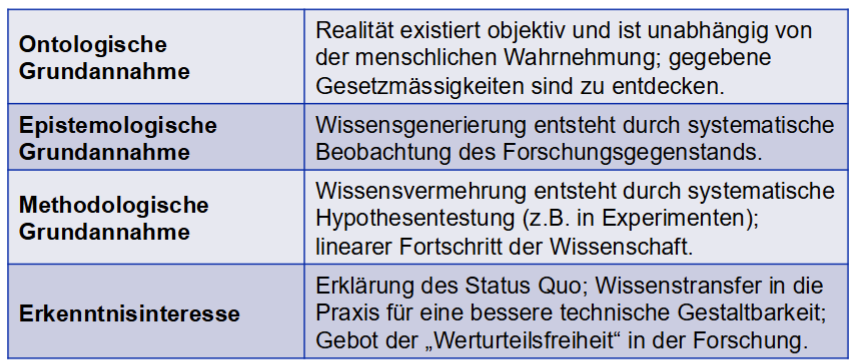
\includegraphics[width=\textwidth,height=0.7\textheight,keepaspectratio]{figures/Naturwissenchaftlich.png}

 \pagebreak
\subsubsection{Interpretativ}
\begin{itemize}
    \item Hermeneutisch, versucht Sinn den 
    \item Sieht soziale Organisationsformen als Resultat politisch-kulturelle Prozesse
    \item Trennung der Objektiven Wirklichkeit in First-Order (Natur <-> Individuum) und Second-order (N-Inviduen <-> First-order reality)
    \item Das Verstehen des Sinns von Handlungen entstehe in Austausch zwischen Forschenden und Subjekten
    \item Gegenstand: Subjektive Wahrnehmung
    \item Methoden: Interviews, Interpretation der Aussagen.
\end{itemize}
\textbf{Profil} \break
 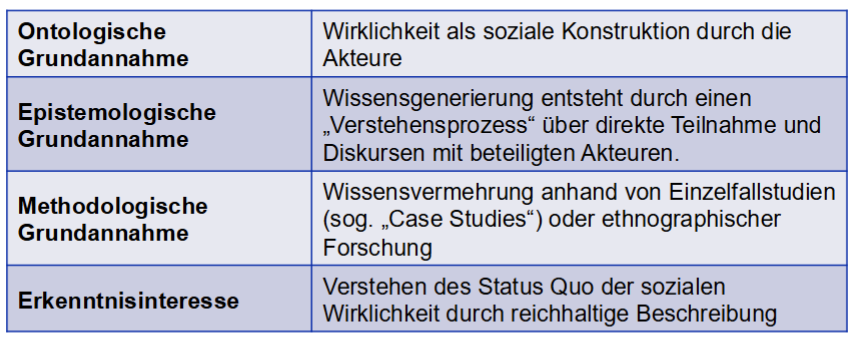
\includegraphics[width=\textwidth,height=0.7\textheight,keepaspectratio]{figures/Interpretativ.png}
 \pagebreak
\subsubsection{Kritisch}
\begin{itemize}
    \item Ziele:
    \begin{itemize}
        \item Kritische Auseinandersetzung mit gegebenen Sozialen Ordnungnen/Organisationen und praktische Veränderung
        \item Herschafftsfreien Diskurs als Mittel zur Konsensbildung über Fragen der Wahrheit und Gerechtigkeit
    \end{itemize} 
    \item Geht den beiden anderen Methoden hinaus mit der 
    \item Annahme: soziale Ordnung ist nicht von Naturgegeben sondern sozial und kulturell bestimmt.
    \item Methode: Geschichtliche Forschrung, Interviews, Analyse Machtverhältnisse
\end{itemize}
\textbf{Profil} \break
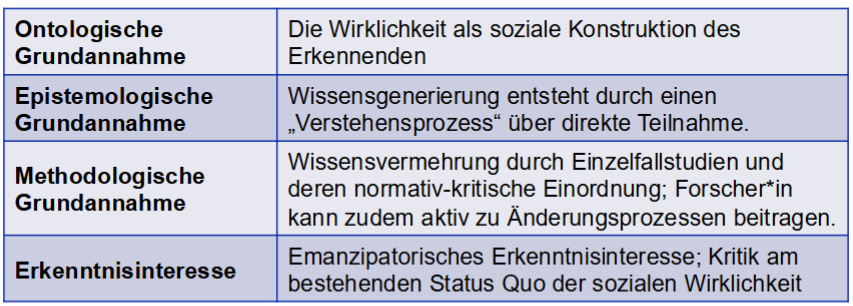
\includegraphics[width=\textwidth,height=0.7\textheight,keepaspectratio]{figures/Kritik.png}
\subsubsection{Vergleich}
Alle Ansätze sollen je nach gegebenen Bedingungen als Werkzeuge zur Analyse verwendet werden. \break
 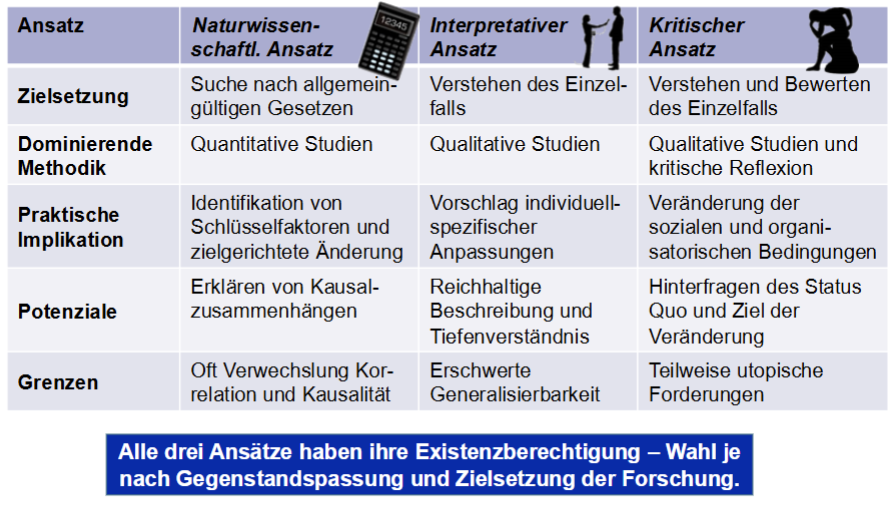
\includegraphics[width=\textwidth,height=0.7\textheight,keepaspectratio]{figures/Vergleich_Ansaetze.png}
 
